\documentclass[utf8]{beamer} \usetheme{lfcr} % Use metropolis theme

\usepackage[brazil,english,francais]{babel}

\usepackage{natbib} \setcitestyle{round}

\usepackage{lmodern} \usepackage{datetime}

\usepackage{ulem}

\usepackage{tikz} \usetikzlibrary{shapes.geometric, arrows, shapes.misc,
  shadows.blur} \usepackage[most]{tcolorbox}

\usepackage{xcolor}

%%%% Defining colors
\definecolor{RoyalBlue}{rgb}{0.0, 0.14, 0.4} \definecolor{OliveGreen}{rgb}{0.33,
  0.42, 0.18} \definecolor{Burgundy}{rgb}{0.5, 0.0, 0.13}
\definecolor{Black}{rgb}{0.0, 0.0, 0.0} \definecolor{Blue}{rgb}{0.0, 0.53, 0.74}

\usepackage{natbib}

\usepackage{graphicx} % Allows including images
\usepackage{booktabs} % Allows the use of \toprule

\usepackage{subfig} \usepackage{stackengine}

\usepackage{float}
\usepackage{placeins} %Binds figures to its respective sections

\usepackage{cases}

\usepackage{varwidth}

\usepackage{multirow}

\usepackage{textcomp} %Text Com­n­in fonts, which pro­vie many text
% sym­ols (such as baht, bul­lt, copy­riht, mu­si­cl­icalnote,
% onequar­er, sec­ton, and yen), in the TS1 en­cocoding.

\usepackage{algpseudocode}

\usepackage{hyperref}

\usepackage{pgfgantt} % Gantt charts - for planning

\setbeamerfont{section in toc}{size=\normalsize}
\setbeamerfont{subsection in toc}{size=\small}

\setbeamercovered{transparent} % For transparency effects with overlay commands
%
%
%
%% figure files' paths
\graphicspath{%
  {../KitPartenairesUPPA/}% logo UPPA
  {../logos/}% misc logos
  {Figures/} {Figures/stateofart/} {Figures/imglabo/} {Figures/setupvalidation/}}

\title{ \vspace*{-1cm} Thesis Report of the: Ongoing experimental research on seismo-electromagnetic fields generated at saturated porous media interfaces}
\date{\today} \author{Victor MARTINS GOMES \\[3mm] Daniel BRITO (PhD supervisor)
  \\ \and H\'{e}l\`{e}ne BARUCQ (PhD co-supervisor)}
\begin{document}
\begin{frame}
  \titlepage
\end{frame}
%
\begin{frame}{Overview}
  \tableofcontents
\end{frame}

%
\section{Introduction}

\begin{frame}{Introduction}
  \textbf{Seismo-electromagnetic phenomena}
  \begin{center}
    \begin{columns}
      \begin{column}{0.7\textwidth}
        \includegraphics[width=0.75\textwidth]{SE_phenomena.pdf}
      \end{column}
      \begin{column}{0.4\textwidth}
        \includegraphics[width=\textwidth]{grainssand.pdf}
      \end{column}
    \end{columns}
  \end{center}
\end{frame}
%
\begin{frame}{Introduction}
  \begin{center}
        \textbf{Interface response:}
        \begin{itemize}
          \item Synchronous
          \item Arrival time is equal to travel time of P-wave to the interface
          \item Max amplitude in receivers whise offset is equal to help the interface depth
          \item Different polarity in source sides
        \end{itemize}

        \rule{\textwidth}{1pt}

    \textbf{Physical properties:}
    Porosity ($\phi$), Permeability ($k_{0}$), Bulk modulus ($K_{s}$,$K_{f}$,$K_{fr}$), frame's Shear
    modulus, densities ($\rho_{s}$,$\rho_{f}$), fluid's electrical conductivity ($\sigma$),
    fluid's viscosity ($\eta$), molarity, temperature, solid and fluid's relative
    permittivity and tortuosity.
  \end{center}
\end{frame}%
%
\begin{frame}{Introduction}

  \textbf{Motivation}

  \begin{itemize}
    \item Hydrocarbon
    \item Bedrock
    \item Water
    \item Water table
    \item CO2 storage
    \item Borehole and surface
  \end{itemize}

\end{frame}
%
\begin{frame}{Introduction}
  \textbf{Motivation}

  \vspace{3.5cm}

  \begin{center}
    \includegraphics[width=\textwidth]{2018Butleretal_Ex_Field.png}
  \end{center}

  \begin{flushleft}
    {\small Butler et al., 2018}
  \end{flushleft}


\end{frame}
%
\section{Experiments: What has been done}
\begin{frame}{Experiments: What has been done}
  \begin{center}
    \textbf{Summary}
   
    \begin{enumerate}
      \item \href{https://library.seg.org/doi/10.1190/1.1620625}{Zhu and Toksöz (2003)}
      \item \href{https://academic.oup.com/jge/article/2/3/222/5127595}{Chen and Mu (2005)}
      \item \href{https://library.seg.org/doi/10.1190/1.2952570}{Zu et al. (2008)}
      \item \href{https://library.seg.org/doi/10.1190/1.3592984}{Schakel et al. (2011)}
      \item \href{https://academic.oup.com/gji/article-abstract/210/3/1703/3867307?redirectedFrom=fulltext}{Peng et al. (2017)}
      \item Ellouz (2017)
    \end{enumerate}
  \end{center}
\end{frame}
%
\begin{frame}{Experiments: What has been done}
  {\textbf{Zhu and Toksöz (2003)}}

  \includegraphics[width=0.3315\textwidth]{Zhu_and_Toksoz_a_fig3}%
  \includegraphics[width=0.3315\textwidth]{Zhu_and_Toksoz_a_fig1}%
  \includegraphics[width=0.3315\textwidth]{Zhu_and_Toksoz_a_fig2}%

  \begin{itemize}
    \item Crosshole w/ water filled fracture
    \item Study fracture aperture vs amplitude
    \item Geometrical parameters of dipping fractures
  \end{itemize}

\end{frame}
%
\begin{frame}{Experiments: What has been done}
  {\textbf{Chen and Mu (2005)}}

  \begin{columns}
    \begin{column}{0.5\textwidth}
      \includegraphics[width=\textwidth]{Chen_and_Mu_a_fig1}%

      \begin{itemize}
        \item NaCl-saturated sand
        \item Salt-water/Water/Oil saturated layers
        \item Conductivity behaviour
          \item converted EM is sensitive to Oil/salt-water
      \end{itemize}
     
    \end{column}
    \begin{column}{0.5\textwidth}
      \includegraphics[angle=-90,origin=c,width=0.5\textwidth]{Chen_and_Mu_a_fig2}%
      \includegraphics[angle=-90,origin=c,width=0.5\textwidth]{Chen_and_Mu_a_fig3}%
    \end{column}
  \end{columns}

\end{frame}
%
\begin{frame}{Experiments: What has been done}
  {\textbf{Zhu et al. (2008)}}

  \begin{columns}
    \begin{column}{0.5\textwidth}
      \includegraphics[width=0.9\textwidth]{Zhuetal2008_b_1}%

      \begin{itemize}
        \item {\small Sandstone and Granite}
        \item {\small Coup Coef for 15 -- 150 kHz}
        \item {\small Coup Coef for Capillary model}
        \item {\small Similar in frequency}
        \item {\small Converted energy $\propto$ Permeabilty and Porosity}

      \end{itemize}

    \end{column}

    \begin{column}{0.5\textwidth}
      \includegraphics[width=0.9\textwidth]{Zhuetal2008_b_2}%

      \includegraphics[width=0.9\textwidth]{Zhuetal2008_b_3}%
    \end{column}
  \end{columns}
 
\end{frame}
%
\begin{frame}{Experiments: What has been done}
  {\textbf{Schakel et al. (2011)}}

  \begin{columns}
    \begin{column}{0.5\textwidth}
      \includegraphics[width=0.9\textwidth]{Schakeletal2011_1}%

      \begin{itemize}
        \item {\small Amp vs. Conductivity}
        \item {\small $\sigma=$ 1.27e-3 (up), 1.20e-2 (middle), 1.01e-1 (bottom)}
      \end{itemize}

    \end{column}

    \begin{column}{0.5\textwidth}
      \includegraphics[width=0.7\textwidth]{Schakeletal2011_3}%

      \includegraphics[width=0.7\textwidth]{Schakeletal2011_2}%

      \includegraphics[width=0.7\textwidth]{Schakeletal2011_4}%
    \end{column}
  \end{columns}
\end{frame}
%
\begin{frame}{Experiments: What has been done}
  {\textbf{Peng et al. (2017)}}

      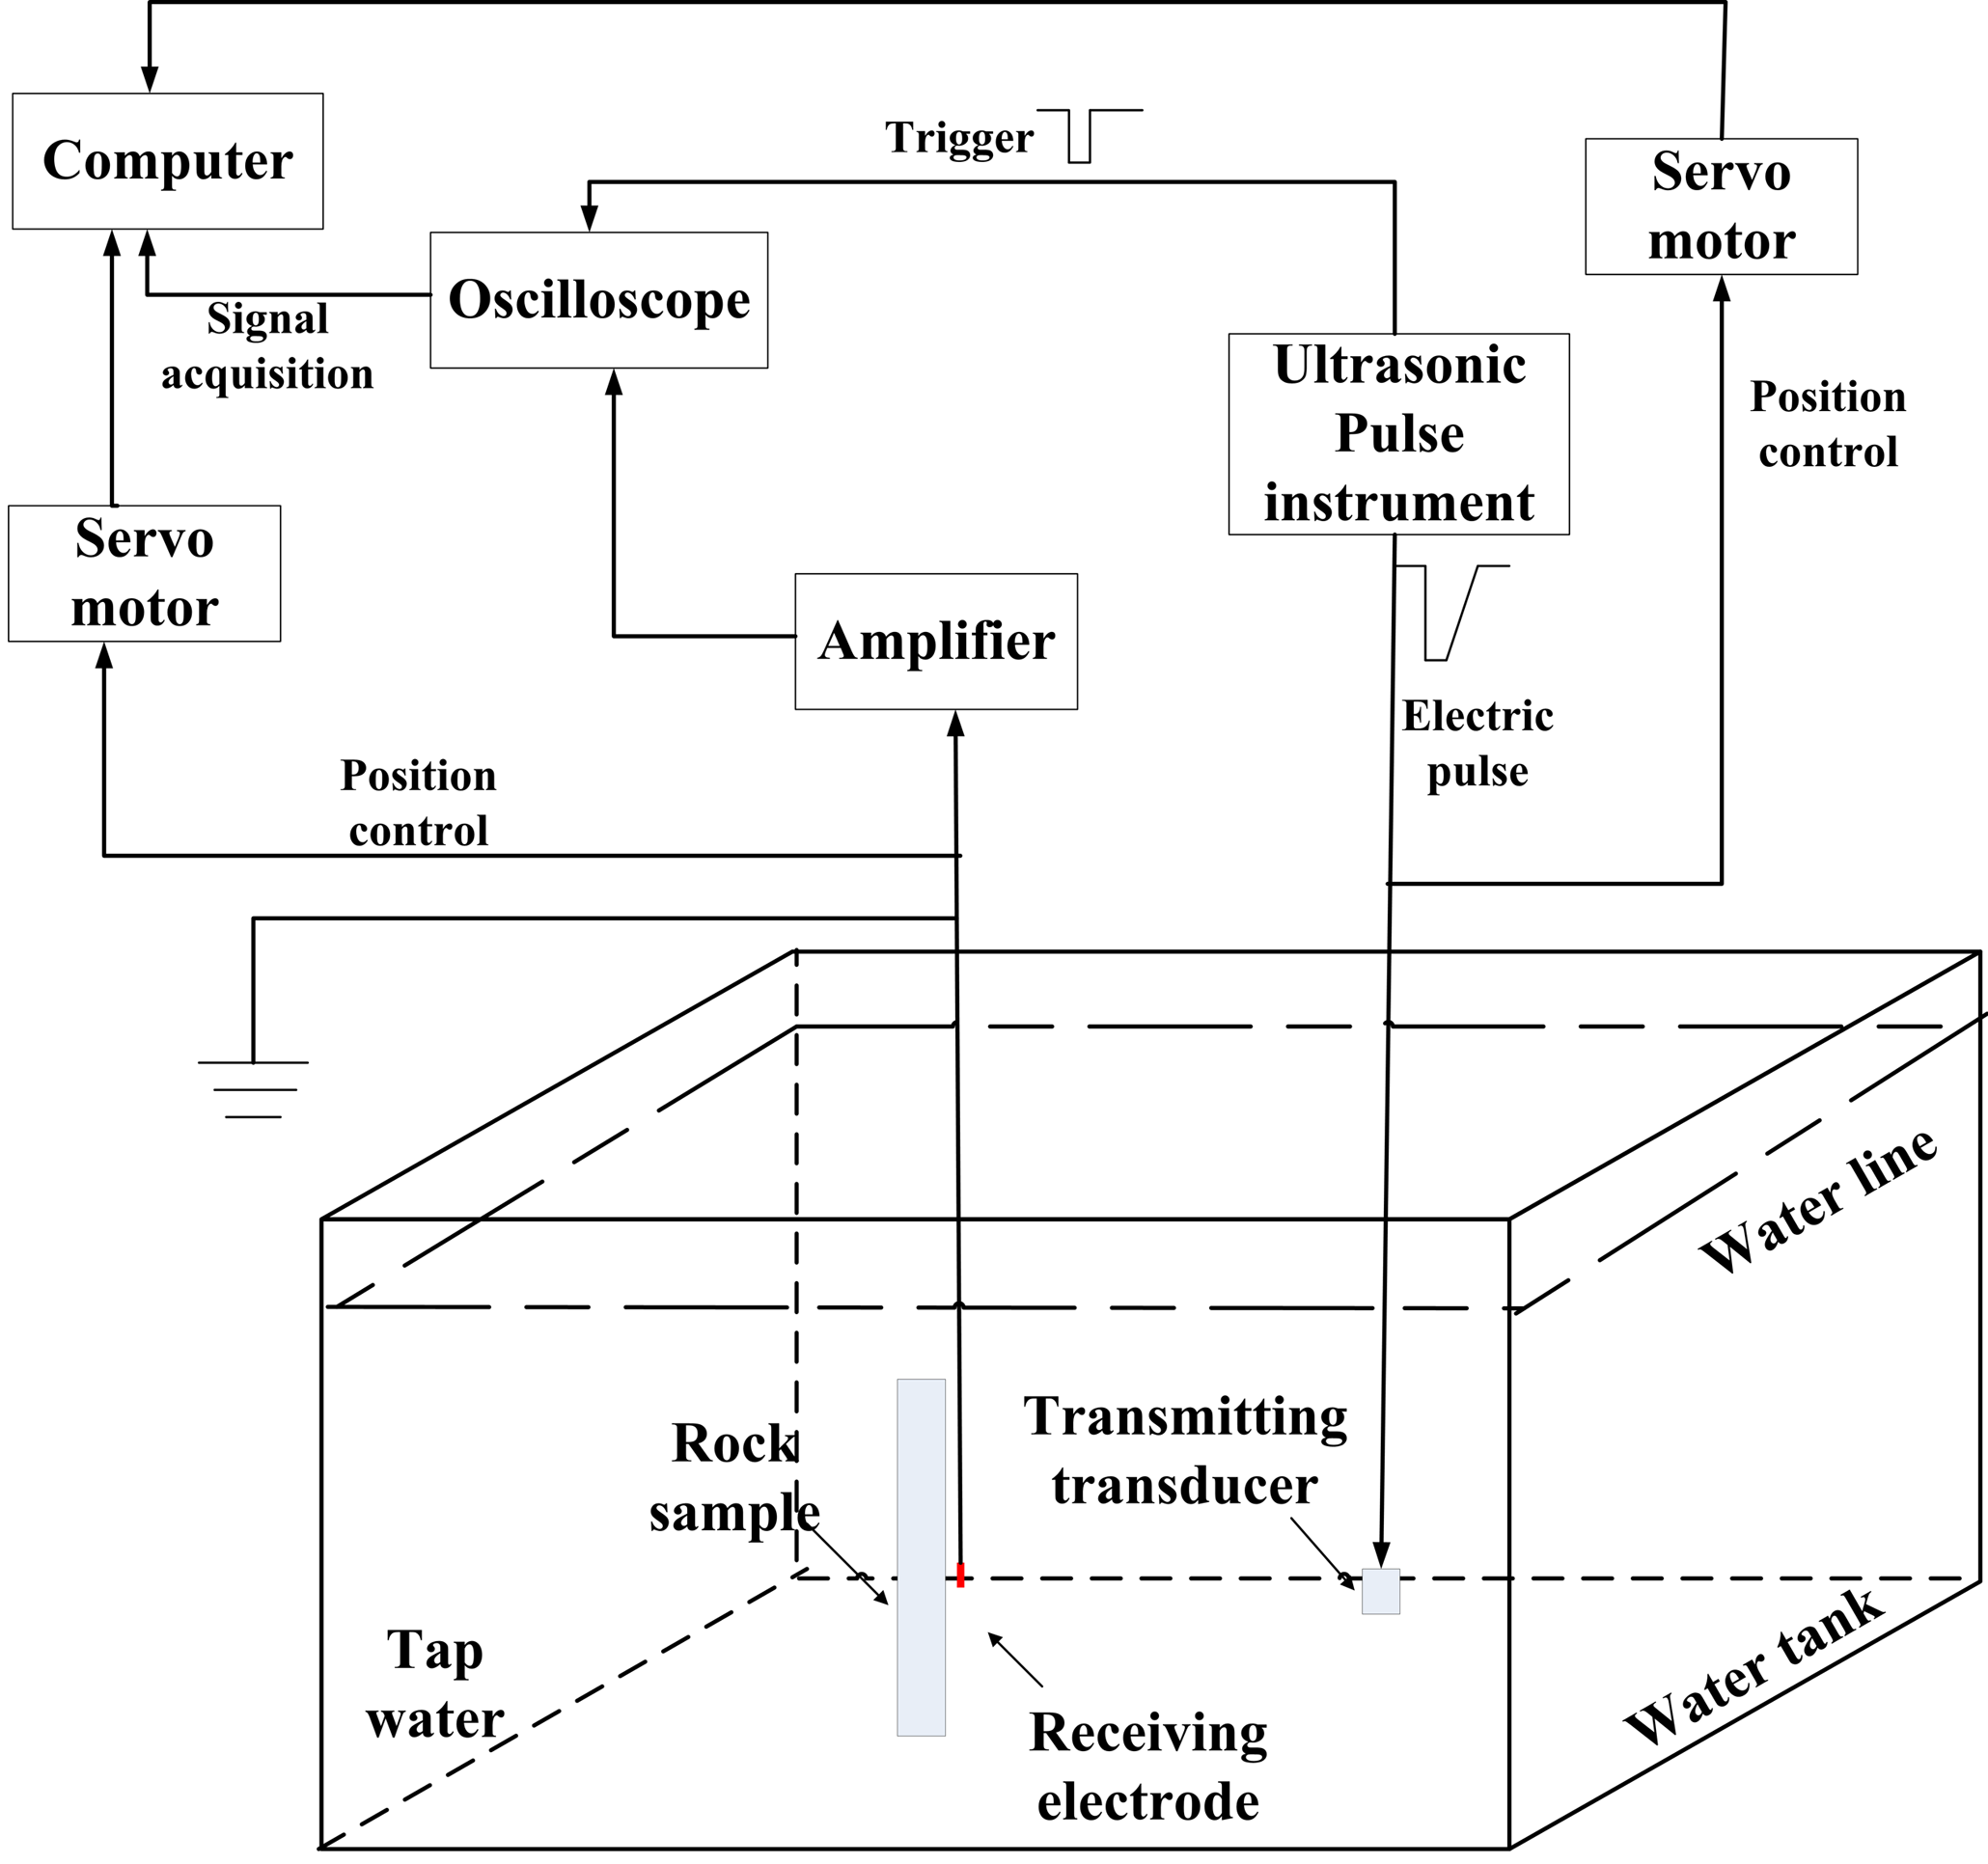
\includegraphics[width=0.4\textwidth]{Pengetal2017_1}%
      \includegraphics[width=0.25\textwidth]{Pengetal2017_2}%
      \includegraphics[width=0.34\textwidth]{Pengetal2017_3}%

      \begin{itemize}
        \item{$\lambda$=0.9cm}
      \end{itemize}
     
\end{frame}
%
\begin{frame}{Experiments: What has been done}
  {\textbf{Peng et al. (2017)}}

  \textbf{Continue:}

      \includegraphics[width=0.4\textwidth]{Pengetal2017_4}%
      \includegraphics[width=0.25\textwidth]{Pengetal2017_5}%
      \includegraphics[width=0.34\textwidth]{Pengetal2017_6}%

      \begin{itemize}
        \item{Experimentally confirmed that thin-layers can enhance the interface response.}
      \end{itemize}

\end{frame}
%
\begin{frame}{Experiments: What has been done}
  {\textbf{Ellouz (2017)}}
  \vspace*{-1cm}
  \begin{block}{}
  \begin{itemize}
    \item {Investigated the effect of various acquisition and geometry-related model parameters to amplitude of converted-EM:

      \begin{itemize}
        \item Thickness
        \item Electrode distance to layer
        \item Excitation frequency

      \end{itemize}
      }
      \item Layer with widths as small as $\lambda/6$ could be identified
  \end{itemize}
  \end{block}

  \vspace*{1.5cm}

  \begin{block}{}
  \includegraphics[width=0.35\textwidth]{ellouz2017_3}
  \end{block}

\end{frame}
%
\begin{frame}{Experiments: What has been done}
  {\textbf{Ellouz (2017)}}

  \begin{center}
    \vspace*{2.5cm}
    \includegraphics[width=0.9\textwidth]{ellouz2017_1}%
  \end{center}

\end{frame}
%
\begin{frame}{Experiments: What has been done}
  {\textbf{Ellouz (2017)}}

  \begin{center}
    \vspace*{2.5cm}
    \includegraphics[width=0.9\textwidth]{ellouz2017_2}%
  \end{center}

  \begin{itemize}
    \item $\lambda \approx $7mm
    \item Thin-layer amplitude enhancement was not seen for 2mm thickness
     
  \end{itemize}

\end{frame}
%
\section{Open questions I will focus}
\subsection{Known questions}
\begin{frame}{Open questions}
  {\textbf{Thin-layers}}
  \begin{center}
  \begin{itemize}
    \item Extend what was experimentally done in Schakel et al. (2012), Peng et al. (2017) and Ellouz (2017)
    \item {Change in thickness and physical properties:
      \begin{itemize}
        \item Wetting fluid/Salinity
        \item Permeability/Porosity
      \end{itemize}
      }
      \item Try to keep up with numerical studies (Grobbe et al., 2016)
  \end{itemize}

  \rule{\textwidth}{1pt}

  \textbf{Thin-layers}: those smaller than the wavelength
  \end{center}
\end{frame}
%
\begin{frame}{Open questions}
  {\textbf{Multi-electrode arrangement}}

  \begin{itemize}
    \item Devi (2017)
      \item 3 and 5-electrodes configuration to reduce noise and amplify EM-waves
  \end{itemize}

  \vspace*{4cm}
  \includegraphics[width=0.9\textwidth]{Devimultielectrode.png}
\end{frame}

\subsection{Questions we have ourselves}
\begin{frame}{Open questions}
  {\textbf{Questions we have ourselves}}

  \begin{block}{\small Reference electrode}

    \vspace*{1.75cm}
    \includegraphics[width=0.9\textwidth]{ref_electrode_config.png}

    \tiny{Ellouz (2017)}
  \end{block}
  \begin{block}{\small Differential amplifier -- Common mode rejection ratio}

    \includegraphics[width=0.5\textwidth]{cmrr.png}
  \end{block}
\end{frame}

%
\section{Experiments to be conducted}
\begin{frame}{Experiments to be conducted}
  \begin{itemize}
    \item {Test:
      \begin{itemize}
        \item Reference electrode (which configuration, are there improvements?, etc.)
        \item Common mode rejection (does it improve our signal? Is it worthy to use it?)
        \item Multi-electrode configuration
      \end{itemize}

      }
    \item Parallel and perpendicular (to layer) measurements
    \item Change rocks /rock properties (heating to change porosity?)
    \item Change wetting fluid ($\mu$m plastic to seal fluid in?)
  \end{itemize}

\end{frame}
%

%
\section{Where am I at?}
\subsection{General view}
\begin{frame}{New experimental set-up}

  \begin{itemize}
    \item Conceived thanks to Federico
    \item With the help of Clarice and Daniel
  \end{itemize}

  \begin{center}
    \includegraphics[width=0.32\textwidth]{Smallcombs_2.PNG}
    \includegraphics[width=0.32\textwidth]{Smallcombs_1.PNG}
    \includegraphics[width=0.32\textwidth]{Bigcomb.PNG}
  \end{center}
 
\end{frame}
%
\begin{frame}{New experimental set-up}
  \begin{columns}
    \begin{column}{0.5\textwidth}
      \textbf{Acoustic-related}

      \includegraphics[width=\textwidth]{newsetup.pdf}
    \end{column}
    \begin{column}{0.5\textwidth}
      \begin{itemize}
        \item Thorlabs equipments
        \item Support for Piezo
        \item Sandbox
      \end{itemize}

    \end{column}
  \end{columns}
\end{frame}
%
\begin{frame}{New experimental set-up}
  \begin{columns}
    \begin{column}{0.5\textwidth}
      \textbf{EM-related}

      \includegraphics[width=\textwidth]{electrodes.pdf}
    \end{column}
    \begin{column}{0.5\textwidth}
      \begin{itemize}
        \item Thicker and longer electrodes
        \item More rigid -> Better positioning
        \item Metallic supportfor moving
      \end{itemize}

    \end{column}
  \end{columns}
\end{frame}
%
\begin{frame}{New experimental set-up}
  \begin{columns}
    \begin{column}{0.5\textwidth}
      \textbf{EM Acquisition-related}

      \includegraphics[width=\textwidth]{IMG_20200224_150608.jpg}
    \end{column}
    \begin{column}{0.5\textwidth}
      \begin{itemize}
        \item Easily make measurements \uline{manually} or in an \uline{automated} way using SPI
        \item Faster acquisitions
        \item Less human influence
      \end{itemize}

    \end{column}
  \end{columns}
\end{frame}
%
\subsection{Automation}
\begin{frame}{Automation -- general view}
  \textbf{Schema}
  \begin{center}
    \includegraphics[width=0.85\textwidth]{schema.pdf}
  \end{center}

\end{frame}

\begin{frame}{Automation -- general view}
  \textbf{Main points}
  \begin{itemize}
   \item {Python-based routines and interface to control the electric acquisition}
    \item {Quicker and simpler acquisition}
    \item {Less human interaction}
    \item {Towards reproductibility}
  \end{itemize}
\end{frame}
%
\subsection{Validation of set-up}
\begin{frame}{Validation}
  {EM-related}
  \textbf{Testing the card}

  \begin{columns}
    \begin{column}{0.5\textwidth}
      \includegraphics[width=\textwidth]{Before_HFnoise_norelayopen.pdf}
      \includegraphics[width=\textwidth]{Before_HFnoise_relayopen.pdf}
    \end{column}
    \begin{column}{0.5\textwidth}
      \includegraphics[width=\textwidth]{Before_HFnoise_ampspec1.pdf}
      \includegraphics[width=\textwidth]{Before_HFnoise_ampspec2.pdf}
    \end{column}
  \end{columns}

\end{frame}
%
\begin{frame}{Validation}
  {EM-related}
  \vspace*{-.5cm}
  \textbf{Testing the card}

  \vspace*{2.5cm}
  \hspace*{3cm}
  \includegraphics[width=0.8\textwidth]{alimentationcircuit.png}


  \begin{columns}
    \begin{column}{0.5\textwidth}
      \includegraphics[width=0.7\textwidth]{converter.jpg}
    \end{column}
    \begin{column}{0.5\textwidth}
      \begin{itemize}
        \item Problem in switching regulator
        \item Solution: remove it
      \end{itemize}
    \end{column}
  \end{columns}

\end{frame}
%
\begin{frame}{Validation}
  {EM-related}
  \textbf{Testing the card}

  \begin{columns}
    \begin{column}{0.5\textwidth}
      \includegraphics[width=\textwidth]{After_HFnoise_norelayopen.pdf}
      \includegraphics[width=\textwidth]{After_HFnoise_relayopen.pdf}
    \end{column}
    \begin{column}{0.5\textwidth}
      \includegraphics[width=\textwidth]{After_HFnoise_ampspec1.pdf}
      \includegraphics[width=\textwidth]{After_HFnoise_ampspec2.pdf}
    \end{column}
  \end{columns}

\end{frame}
%
\begin{frame}{Validation}
  {EM-related}
  \textbf{Testing electrodes}
  \begin{center}
    \includegraphics[width=0.475\textwidth]{maxperdriverrelay.pdf}
    \includegraphics[width=0.475\textwidth]{ampperelectrode.pdf}
  \end{center}
 
\end{frame}
%
\begin{frame}{Validation}
  {EM-related}
  \textbf{Testing electrodes}

  \begin{columns}
    \begin{column}{0.5\textwidth}
      \begin{itemize}
        \item Some defectuous electrodes in two combs
        \item Long comb (2,5,7,18 and 24)
        \item Short comb (9,24,26,27 and 31)
        \item Not yet solved
      \end{itemize}
    \end{column}
    \begin{column}{\textwidth}
        \includegraphics[width=0.5\textwidth]{peigne_long.jpg}
    \end{column}
  \end{columns}

\end{frame}
%
%%%%
\subsection{Planning validation and automation}
\begin{frame}{Automation and validation Planning}
  \textbf{From: 2020-01-30 until 2020-03-13}

  \vspace*{0.5cm}
  \hspace*{-0.5cm}
  \resizebox{11.5cm}{!}{
	\begin{ganttchart}[ x unit=0.45cm, y unit title=0.7cm, y unit chart=0.9cm,
      vgrid={draw=none, dotted}, time slot format=isodate, time slot unit=day,
      calendar week text = {W\currentweek{}}, title/.append style={draw=none,
        fill=RoyalBlue!50!black}, title label font=
      \sffamily\bfseries\Large\color{white}, title label node/.append
      style={below=-1.6ex}, title left shift=.05, title right shift=-.05, title
      height=1, bar/.append style={draw=none, fill=OliveGreen!75}, bar
      height=.6, bar label font=\Large\color{black!80}, group right shift=0,
      group top shift=.6, group height=.3, group peaks height=.2, group label
      font=\sffamily\bfseries\LARGE\color{black}, bar incomplete/.append
      style={fill=Burgundy}, bar progress label font=\Large\color{Black}, group
      progress label font=\Large\color{Black}, milestone progress label
      font=\Large\color{Black}, milestone label font=\Large\color{Blue}, bar
      progress label font=\Large\color{Black}, progress=today, today=2020-02-20
      ]{2020-01-30}{2020-03-13}
      \gantttitlecalendar{year, month=name, week} \\
      \ganttbar[ bar progress label font=\Large\color{OliveGreen!75}, bar
      progress label node/.append style={right=4pt}, progress=40, bar label
      font=\LARGE\color{OliveGreen}, name=pp
      ]{Overall}{2020-01-30}{2020-03-13} \\
      \ganttset{link/.style={black, thick, -to}} \ganttbar[name=osc,
      progress=70]{Oscilloscope}{2020-01-30}{2020-03-13} \\
      \ganttbar[name=elec,
      progress=50]{Elec. card}{2020-01-30}{2020-03-13} \\
      \ganttbar[name=las,
      progress=90]{Acoustic}{2020-01-30}{2020-03-13} \\
      \ganttbar[name=tava
      progress=30]{Tests and vali.}{2020-01-30}{2020-03-13} \\
	\end{ganttchart}
  }
  \begin{itemize}
    \item \textcolor{red}{\bf \* Proposed at 2020-02-20}
  \end{itemize}
\end{frame}
%
\begin{frame}{Automation and validation Planning}
  \textbf{Today}

  \vspace*{0.5cm}
  \hspace*{-0.5cm}
  \resizebox{11.5cm}{!}{
	\begin{ganttchart}[ x unit=0.45cm, y unit title=0.7cm, y unit chart=0.9cm,
      vgrid={draw=none, dotted}, time slot format=isodate, time slot unit=day,
      calendar week text = {W\currentweek{}}, title/.append style={draw=none,
        fill=RoyalBlue!50!black}, title label font=
      \sffamily\bfseries\Large\color{white}, title label node/.append
      style={below=-1.6ex}, title left shift=.05, title right shift=-.05, title
      height=1, bar/.append style={draw=none, fill=OliveGreen!75}, bar
      height=.6, bar label font=\Large\color{black!80}, group right shift=0,
      group top shift=.6, group height=.3, group peaks height=.2, group label
      font=\sffamily\bfseries\LARGE\color{black}, bar incomplete/.append
      style={fill=Burgundy}, bar progress label font=\Large\color{Black}, group
      progress label font=\Large\color{Black}, milestone progress label
      font=\Large\color{Black}, milestone label font=\Large\color{Blue}, bar
      progress label font=\Large\color{Black}, progress=today, today=2020-04-24
      ]{2020-01-30}{2020-04-24}
      \gantttitlecalendar{year, month=name, week} \\
      \ganttbar[ bar progress label font=\Large\color{OliveGreen!75}, bar
      progress label node/.append style={right=4pt}, progress=80, bar label
      font=\LARGE\color{OliveGreen}, name=pp
      ]{Overall}{2020-01-30}{2020-04-24} \\
      \ganttset{link/.style={black, thick, -to}} \ganttbar[name=osc,
      progress=90]{Oscilloscope}{2020-01-30}{2020-03-13} \\
      \ganttbar[name=elec,
      progress=90]{Elec. card}{2020-01-30}{2020-03-13} \\
      \ganttlinkedbar[name=spi,
      progress=100]{SPI connection}{2020-02-20}{2020-02-28}\\
      \ganttlinkedbar[name=tnoise,
      progress=100]{Transformer noise}{2020-03-02}{2020-03-11}\\
      \ganttlinkedbar[name=eletr,
      progress=50]{Electrodes}{2020-03-02}{2020-03-16}\\
      \ganttbar[name=lasa
      progress=50]{Acoustic}{2020-01-30}{2020-03-13} \\
      \ganttbar[name=tav,
      progress=85]{Tests and vali.}{2020-01-30}{2020-04-24} \\
	\end{ganttchart}
  }

\end{frame}%
%
\begin{frame}{Tests yet to be performed}
  \begin{itemize}
    \item {Test box attenuation/plastic velocity/etc \textcolor{blue}{ONGOING}
      \begin{itemize}
        \item Better characterize measurements
          \item More measurements
      \end{itemize}
      }
    \item Sand-filled box
    \item Sensitivity to the Layer response
    \item Check for improvements (acoustic and electric-wise) from previous experiment
  \end{itemize}
\end{frame}
%
\subsection{Perspectives}
\begin{frame}{Perspectives to new experimentl setup}
  \textbf{General:}
  \begin{enumerate}
    \item Greater SNR
    \item Faster acquisition
    \item Greater spatial precision of electric measurements due to more rigid
      electrodes
    \item Ensure repeatability
    \item More precision when studying the converted wave
  \end{enumerate}

 \visible<2>{\textbf{In the end: A robust and easily reproducible seismoelectric experiment.}}
\end{frame}
%
\section{Planning}
%
\begin{frame}{Final Planning}
  \textbf{Today}

  \vspace*{0.5cm}
  \hspace*{-0.5cm}
  \resizebox{11.5cm}{!}{
	\begin{ganttchart}[ x unit=0.45cm, y unit title=0.7cm, y unit chart=0.9cm,
      vgrid={draw=none, dotted}, time slot format=isodate, time slot unit=day,
      calendar week text = {W\currentweek{}}, title/.append style={draw=none,
        fill=RoyalBlue!50!black}, title label font=
      \sffamily\bfseries\Large\color{white}, title label node/.append
      style={below=-1.6ex}, title left shift=.05, title right shift=-.05, title
      height=1, bar/.append style={draw=none, fill=OliveGreen!75}, bar
      height=.6, bar label font=\Large\color{black!80}, group right shift=0,
      group top shift=.6, group height=.3, group peaks height=.2, group label
      font=\sffamily\bfseries\LARGE\color{black}, bar incomplete/.append
      style={fill=Burgundy}, bar progress label font=\Large\color{Black}, group
      progress label font=\Large\color{Black}, milestone progress label
      font=\Large\color{Black}, milestone label font=\Large\color{Blue}, bar
      progress label font=\Large\color{Black}, progress=today, today=2020-04-24
      ]{2020-04-24}{2020-07-31}
      \gantttitlecalendar{year, month=name, week} \\
      \ganttbar[ bar progress label font=\Large\color{OliveGreen!75}, bar
      progress label node/.append style={right=4pt}, progress=10, bar label
      font=\LARGE\color{OliveGreen}, name=pp
      ]{Thesis redaction}{2020-04-24}{2020-07-31} \\
      \ganttset{link/.style={black, thick, -to}} \ganttbar[name=osc,
      progress=90]{Automation}{2020-04-24}{2020-05-20} \\
      \ganttlinkedbar[name=eletr,
      progress=50]{Electrodes}{2020-04-24}{2020-05-16}\\
      \ganttbar[name=tav,
      progress=85]{Tests and vali.}{2020-05-11}{2020-06-03} \\
      \ganttlinkedbar[name=eletr,
      progress=50]{Electrodes}{2020-05-11}{2020-05-16}\\
      \ganttlinkedbar[name=CompE,
      progress=20]{Comp w/ Ellouz data}{2020-05-11}{2020-06-03}\\
      \ganttbar[name=main,
      progress=0]{Main topic}{2020-06-01}{2020-07-31} \\
      \ganttlinkedbar[name=cmrr,
      progress=0]{Differential amplifier}{2020-06-01}{2020-06-12}\\
      \ganttlinkedbar[name=rfelc,
      progress=0]{Ref. electrodes}{2020-06-01}{2020-06-12}\\
      \ganttlinkedbar[name=mfelc,
      progress=0]{Mult. electrodes}{2020-06-01}{2020-06-12}\\
      \ganttlinkedbar[name=firstexp,
      progress=0]{Exp. after Ellouz}{2020-06-09}{2020-06-26}\\
      \ganttlinkedbar[name=thick,
      progress=0]{Layer thickness}{2020-06-29}{2020-07-03}\\
      \ganttlinkedbar[name=wet,
      progress=0]{Wetting fluid}{2020-07-06}{2020-07-10}\\
      \ganttlinkedbar[name=porper,
      progress=0]{Change rock}{2020-07-13}{2020-07-17}\\
      \ganttbar[name=expp,
      progress=0]{Experimental planning}{2020-06-01}{2020-07-31} \\
      \ganttbar[name=dat,
      progress=0]{Data analysis}{2020-06-01}{2020-07-31} \\

	\end{ganttchart}
  }

\end{frame}%

%%%%%%%%%%%%%%%%%%%%%%%%%%%%%%%%%%%%%%%%%%%%%%%%%%%%%%%%%%%%%%%%%%%%%%%%%
  
  %%%%%%%%%%%%%%%%%%%%%%%
% DO NOT CHANGE BELOW %
  %%%%%%%%%%%%%%%%%%%%%%%
\begin{frame}{}
  \centering
  \begin{beamercolorbox}[wd=\paperwidth, ht=1.2cm]{frametitle}
    \begin{tikzpicture}
      \useasboundingbox(0,0) rectangle(\the\paperwidth,1.5); {
        \draw[preaction={fill=black,opacity=.4,transform
          canvas={xshift=0.0mm,yshift=-0.5mm}}][draw=white,fill=myblue]
        (-0.1,-1) -- (-0.1,1.5) -- (19,1.5) -- (19,-0.25); \node[anchor=base] at
        (6.12875,0) {\usebeamerfont{frametitle}\huge Thank you for your
          attention!}; }
    \end{tikzpicture}
  \end{beamercolorbox}
\end{frame}

\end{document}
